\section{Peterson and Hamilton algorithm - Modeling,  Specification and Testing}
% no \IEEEPARstart


Peterson's algorithm (aka Peterson's solution) is a concurrent programming algorithm for mutual exclusion. Mutual exclusion (often abbreviated to mutex) algorithms are used in concurrent programming to avoid the simultaneous use of a common resource, such as a global variable, by pieces of computer code called critical sections. A critical section is a piece of code in which a process or thread accesses a common resource. The critical section by itself is not a mechanism or algorithm for mutual exclusion. A program, process, or thread can have the critical section in it without any mechanism or algorithm which implements mutual exclusion. Assume that a variable (memory location) can only have one value (never between values) and processes A and B write want to write to the same memory location at the "same time", either the value from A or the value from B will be written rather than some scrambling of bits. Peterson and Hamilton's algorithm is a simple algorithm that can be run by two processes to ensure mutual exclusion for one resource (say one variable or data structure). Shared variables are created and initialized before either process starts. The shared variables flag[0] and flag[1] are initialized to FALSE because neither process is yet interested in the critical section. The shared variable turn is set to either 0 or 1 randomly (or it can always be set to say 0). The next figure shows the algorithm.

\begin{figure}[h!]
var flag: array [0..1] of boolean; \\*
turn: 0..1; \\*
//flag[k] means that process[k] is interested in the critical section \\*
flag[0] := FALSE; \\*
flag[1] := FALSE; \\*
turn := random(0..1) \\*
//After initialization, each process, which is called process i in the code, runs this code: \\*
repeat \\
\begin{tabular} l
 flag[i] := TRUE; \\*
 turn := j; \\*
 while (flag[j] and turn=j) do no-op; \\*
 //CRITICAL SECTION \\*
 flag[i] := FALSE; \\*
 //REMAINDER SECTION \\*
\end{tabular} \\
until FALSE;\\*
\caption{Peterson-Hamilton's algorithm}
\label{fig:model1}
\end{figure}

There are two different processes which want to enter at critical section. 
This means that the processes are fighting for one resource (ex. Say one variable or data structure). 
flag[i]= true means that process I wants to enter the critical section and the turn=i means that process i is next to enter the critical section.
 At first the shared variables flag[0] and flag[1] are initialized to false because neither process is yet interested in the critical section. 
 The shared variable turn is set to either 0 or 1 randomly (or it can always be set to say 0). 
 If the process can’t enter the critical section it waits in while loop.
\\*
Legend:
turn € {0, 1}
flag0, flag1 € {true, false} = {t, f}
w – write
r – read
enter – enter the critical section
exit – exit the critical section

Initialization:\\*
turn=1\\*
flag1 = flag2 = f\\*

CCS Specification:\\*
Peterson = (P1 | P2 | flag1f | flag2f | turn1) \ L\\*
P1 = flag1wt.turnw2.P11\\*
P11 = flag2rf.P12 + flag2rt.(turnr2. τ.P11 + turnr1.P12)\\*
P12 = enter1.exit1.flag1wf.P1\\*\\*
P2 = flag2wt.turnw1.P21\\*
P21 = flag1rf.P22 + flag1rt.(turnr1. τ.P21 + turnr2.P22)\\*
P22 = enter2.exit2.flag2wf.P2\\*\\*
FLAG1f = flag1rf.flag1f + flag1wf.flag1f + flag1wt.flag1t\\*
FLAG1t = flag1rt.flag1t + flag1wt.flag1t + flag1wf.flag1f\\*\\*
FLAG2f = flag2rf.flag2f + flag2wf.flag2f + flag2wt.flag2t\\*
FLAG2t = flag2rt.flag2t + flag2wt.flag2t + flag2wf.flag2f\\*
TURN1 = turnr1.turn1 + turnw1.turn1 + turnw2.turn2\\*\\*
TURN2 = turnr2.turn2 + turnw2.turn2 + turnw1.turn1\\*\\*
L = { flag1wt, flag1rt, turnw2,… union of the access sorts (r,w) of the
variables }\\*

\begin{figure}[h!]
\centering
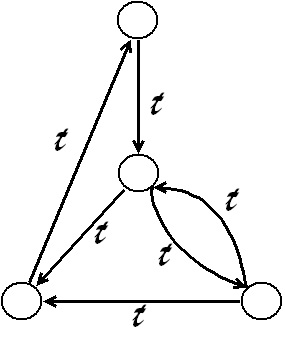
\includegraphics[width=1.0in]{model1}
% where an .eps filename suffix will be assumed under latex, 
% and a .pdf suffix will be assumed for pdflatex; or what has been declared
% via \DeclareGraphicsExtensions.
\caption{Live cycle of one process}
\label{fig:model1}
\end{figure}

\begin{figure}[!ht]
\centering
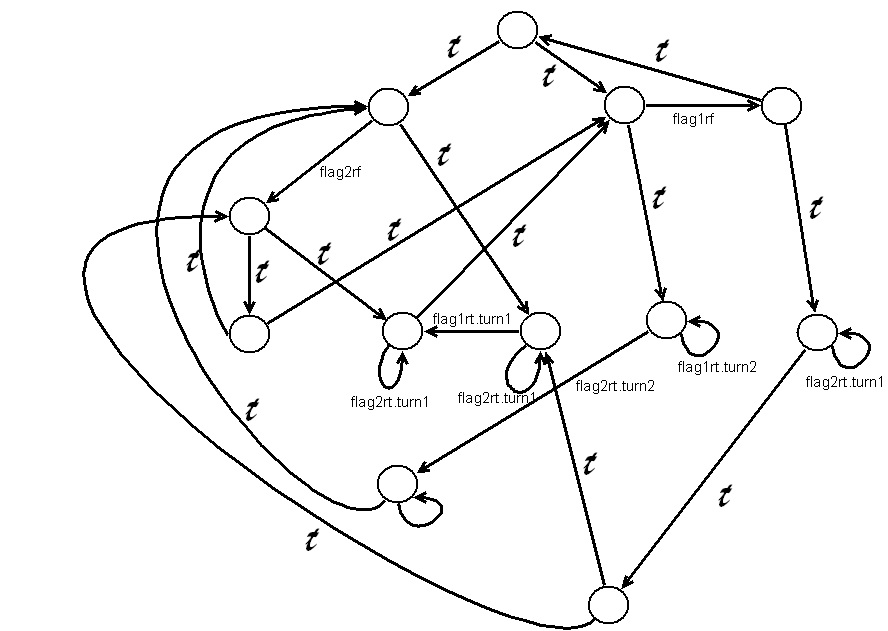
\includegraphics[width=3.5in]{model2}
% where an .eps filename suffix will be assumed under latex, 
% and a .pdf suffix will be assumed for pdflatex; or what has been declared
% via \DeclareGraphicsExtensions.
\caption{Model of Peterson-Hamilton algorithm}
\label{fig:model2}
\end{figure}

The previous figures were shown pictures of life cycle of a one process and Model of Peterson - Hamilton algorithm.

The mutual exclusion requirement is assured. Suppose instead that both processes are in their critical section. 

Only one can have the turn, so the other must have reached the while test before the process with the turn set its flag. 
But after setting its flag, the other process had to give away the turn. 
Contradicting our assumption, the process at the while test has already changed the turn and will not change it again.
	The progress requirement is assured. 
	
	Again, the turn variable is only considered when both processes are using, or trying to use, the resource.
	Deadlock is not possible. One of the processes must have the turn if both processes are testing the while condition. 
	That process will proceed.
	Finally, bounded waiting is assured. When a process that has exited the CS reenters, it will give away the turn. 
	If the other process is already waiting, it will be the next to proceed.\\*

Test and set algorithm\\*
repeat\\*
while Test-and-Set(lock) do no-op;\\*
critical section \\*
lock := false;\\*
remainder section \\*
until false \\*\\*
Test-and-Set(target) \\*
result := target;\\*
target := true; \\*
return result \\*\\*
\begin{tabular}{ |p{4.0cm}| p{4.0cm} | }
  \hline                       
  Process 1	& Process 2 \\ \hline 
  Wants to set target to true & \\
  Target is changed to true & \\
  Result comes back false so no busy waiting &\\
  & Wants to set target to true \\
  & It receives the result true \\
  & Busy waits as long as Process 1 is in critical section \\
  Leaves critical section & \\
  Set target to false & \\
  \hline  
\end{tabular}
